\documentclass[11pt,compress,t,notes=noshow, xcolor=table]{beamer}
\usepackage[]{graphicx}\usepackage[]{color}
% maxwidth is the original width if it is less than linewidth
% otherwise use linewidth (to make sure the graphics do not exceed the margin)
\makeatletter
\def\maxwidth{ %
  \ifdim\Gin@nat@width>\linewidth
    \linewidth
  \else
    \Gin@nat@width
  \fi
}
\makeatother

\newcommand{\citebutton}[2]{%
\beamergotobutton{\href{#2}{#1}}%
}

\newcommand{\blu}[1]{\textcolor{blue}{#1}}
\newcommand{\org}[1]{\textcolor{orange}{#1}}
\newcommand{\ques}{\textbf{\textcolor{red}{Question:  }}}
\newcommand{\questionssofar}{\begin{frame}\frametitle{Any questions?}\end{frame}}

\newcommand\warning{%
 \makebox[1.4em][c]{%
 \makebox[0pt][c]{\raisebox{.1em}{\scriptsize!}}%
 \makebox[0pt][c]{\color{red}\normalsize$\bigtriangleup$}}}%

\definecolor{fgcolor}{rgb}{0.345, 0.345, 0.345}
\newcommand{\hlnum}[1]{\textcolor[rgb]{0.686,0.059,0.569}{#1}}%
\newcommand{\hlstr}[1]{\textcolor[rgb]{0.192,0.494,0.8}{#1}}%
\newcommand{\hlcom}[1]{\textcolor[rgb]{0.678,0.584,0.686}{\textit{#1}}}%
\newcommand{\hlopt}[1]{\textcolor[rgb]{0,0,0}{#1}}%
\newcommand{\hlstd}[1]{\textcolor[rgb]{0.345,0.345,0.345}{#1}}%
\newcommand{\hlkwa}[1]{\textcolor[rgb]{0.161,0.373,0.58}{\textbf{#1}}}%
\newcommand{\hlkwb}[1]{\textcolor[rgb]{0.69,0.353,0.396}{#1}}%
\newcommand{\hlkwc}[1]{\textcolor[rgb]{0.333,0.667,0.333}{#1}}%
\newcommand{\hlkwd}[1]{\textcolor[rgb]{0.737,0.353,0.396}{\textbf{#1}}}%
\let\hlipl\hlkwb

\usepackage{framed}
\makeatletter
\newenvironment{kframe}{%
 \def\at@end@of@kframe{}%
 \ifinner\ifhmode%
  \def\at@end@of@kframe{\end{minipage}}%
  \begin{minipage}{\columnwidth}%
 \fi\fi%
 \def\FrameCommand##1{\hskip\@totalleftmargin \hskip-\fboxsep
 \colorbox{shadecolor}{##1}\hskip-\fboxsep
     % There is no \\@totalrightmargin, so:
     \hskip-\linewidth \hskip-\@totalleftmargin \hskip\columnwidth}%
 \MakeFramed {\advance\hsize-\width
   \@totalleftmargin\z@ \linewidth\hsize
   \@setminipage}}%
 {\par\unskip\endMakeFramed%
 \at@end@of@kframe}
\makeatother

\definecolor{shadecolor}{rgb}{.97, .97, .97}
\definecolor{messagecolor}{rgb}{0, 0, 0}
\definecolor{warningcolor}{rgb}{1, 0, 1}
\definecolor{errorcolor}{rgb}{1, 0, 0}
\newenvironment{knitrout}{}{} % an empty environment to be redefined in TeX

\usepackage{alltt}
\newcommand{\SweaveOpts}[1]{}  % do not interfere with LaTeX
\newcommand{\SweaveInput}[1]{} % because they are not real TeX commands
\newcommand{\Sexpr}[1]{}       % will only be parsed by R
\newcommand{\xmark}{\ding{55}}%


\usepackage[english]{babel}
\usepackage[utf8]{inputenc}

\usepackage{dsfont}
\usepackage{verbatim}
\usepackage{amsmath}
\usepackage{amsfonts}
\usepackage{amssymb}
\usepackage{bm}
\usepackage{csquotes}
\usepackage{multirow}
\usepackage{longtable}
\usepackage{booktabs}
\usepackage{enumerate}
\usepackage[absolute,overlay]{textpos}
\usepackage{psfrag}
\usepackage{algorithm}
\usepackage{algpseudocode}
\usepackage{eqnarray}
\usepackage{arydshln}
\usepackage{tabularx}
\usepackage{placeins}
\usepackage{tikz}
\usepackage{setspace}
\usepackage{colortbl}
\usepackage{mathtools}
\usepackage{wrapfig}
\usepackage{bm}
\usepackage{amsmath}
\usepackage{pifont}

\usetikzlibrary{shapes.multipart,shapes,arrows,automata,positioning,calc,chains,trees, shadows}
\tikzset{
  %Define standard arrow tip
  >=stealth',
  %Define style for boxes
  punkt/.style={
    rectangle,
    rounded corners,
    draw=black, very thick,
    text width=6.5em,
    minimum height=2em,
    text centered},
  % Define arrow style
  pil/.style={
    ->,
    thick,
    shorten <=2pt,
    shorten >=2pt,}
}

\tikzstyle{vec}=[draw, rectangle, fill = white, minimum width=5mm, minimum height=1cm, inner sep = 2pt]

\usepackage{subfig}

% Defines macros and environments
\usepackage{../../style/lmu-lecture}


\let\code=\texttt
\let\proglang=\textsf

\setkeys{Gin}{width=0.9\textwidth}

\setbeamertemplate{frametitle}{\expandafter\uppercase\expandafter\insertframetitle}

\usepackage{bbm}
% basic latex stuff
\newcommand{\pkg}[1]{{\fontseries{b}\selectfont #1}} %fontstyle for R packages
\newcommand{\lz}{\vspace{0.5cm}} %vertical space
\newcommand{\dlz}{\vspace{1cm}} %double vertical space
\newcommand{\oneliner}[1] % Oneliner for important statements
{\begin{block}{}\begin{center}\begin{Large}#1\end{Large}\end{center}\end{block}}


%new environments
\newenvironment{vbframe}  %frame with breaks and verbatim
{
 \begin{frame}[containsverbatim,allowframebreaks]
}
{
\end{frame}
}

\newenvironment{vframe}  %frame with verbatim without breaks (to avoid numbering one slided frames)
{
 \begin{frame}[containsverbatim]
}
{
\end{frame}
}

\newenvironment{blocki}[1]   % itemize block
{
 \begin{block}{#1}\begin{itemize}
}
{
\end{itemize}\end{block}
}

\newenvironment{fragileframe}[2]{  %fragile frame with framebreaks
\begin{frame}[allowframebreaks, fragile, environment = fragileframe]
\frametitle{#1}
#2}
{\end{frame}}


\newcommand{\myframe}[2]{  %short for frame with framebreaks
\begin{frame}[allowframebreaks]
\frametitle{#1}
#2
\end{frame}}

\newcommand{\remark}[1]{
  \textbf{Remark:} #1
}


\newenvironment{deleteframe}
{
\begingroup
\usebackgroundtemplate{
\includegraphics[width=\paperwidth,height=\paperheight]{../style/color/red.png}}
 \begin{frame}
}
{
\end{frame}
\endgroup
}
\newenvironment{simplifyframe}
{
\begingroup
\usebackgroundtemplate{
\includegraphics[width=\paperwidth,height=\paperheight]{../style/color/yellow.png}}
 \begin{frame}
}
{
\end{frame}
\endgroup
}\newenvironment{draftframe}
{
\begingroup
\usebackgroundtemplate{
\includegraphics[width=\paperwidth,height=\paperheight]{../style/color/green.jpg}}
 \begin{frame}
}
{
\end{frame}
\endgroup
}
% https://tex.stackexchange.com/a/261480: textcolor that works in mathmode
\makeatletter
\renewcommand*{\@textcolor}[3]{%
  \protect\leavevmode
  \begingroup
    \color#1{#2}#3%
  \endgroup
}
\makeatother





\input{../../latex-math/basic-math.tex}
\input{../../latex-math/basic-ml.tex}



\newcommand{\titlefigure}{figure/python.png} %TODO
\newcommand{\learninggoals}{
\item Understand how a tensor works
\item Understand how backpropagation works
\item Be able to write basic PyTorch code}

\renewcommand{\bfseries}{\mdseries}





\title{Pytorch Logic}
% \author{}
\institute{\href{https://slds-lmu.github.io/lecture_dl4nlp/}{slds-lmu.github.io/lecture\_dl4nlp}}
\date{}

\begin{document}
\lecturechapter{Exercise 3}
\lecture{Deep Learning for NLP}

% ------------------------------------------------------------------------------

\begin{vbframe}{Why Pytorch?}

\vfill

Can we implement neural networks with numpy?

Sure we can, but...
\vfill
 \begin{itemize}
 \item ... we would have to implement many functionalities from scratch
 \item ... we would have to derive all of our gradients by hand $\rightarrow$ error-prone and annoying
 \item ... numpy has no inherent way of grouping functions and their parameters $\rightarrow$ no modularization
 \item ... numpy does not support calculations on GPU
 \end{itemize}


\vfill

\end{vbframe}

% ------------------------------------------------------------------------------

\begin{vbframe}{Enter pytorch!}

	\vfill
	\begin{itemize}
	 \item Open source library for deep learning with Python, developed by Facebook
	 \item Documentation: \url{http://pytorch.org/docs/master/torch.html}
	 \item 60 minute tutorial: \url{https://pytorch.org/tutorials/beginner/deep_learning_60min_blitz.html}
	\end{itemize}
	

\vfill

\end{vbframe}

\begin{vbframe}{Pytorch}

	\vfill
	\begin{itemize} 
		\item ... has many pre-implemented layers, loss functions and optimizers
		\item ... can do gradients and backpropagation automatically
		\item ... has object-oriented grouping of functions and parameters into modules
		\item ... supports calculations on GPU
	   \end{itemize}
	   
	

\vfill

\end{vbframe}


\begin{vbframe}{Tensors}

	\vfill
	\begin{itemize}
		\item \texttt{torch.tensor}: Numerical objects (scalars, vectors, matrices...)
		 \item Every tensor has a data type (dtype) and a shape (which is called \textit{size})
		\item Tensors can be manipulated and combined via operations (addition, matrix multiplication, concatenation, etc.)
		\item The result of a tensor operation is a new tensor
		\item Think about \texttt{torch.tensor} as the pytorch equivalent of \texttt{numpy.array} (but with some additional abilities related to gradients)
	   \end{itemize}
	   
\vfill

\end{vbframe}


\begin{frame}[fragile]{Creating tensors}
\vfill
\begin{minted}[fontsize=\tiny,fontfamily=courier]{python}
>>> import torch
>>> # You can create tensors from nested Python lists:
>>> torch.tensor([[1.0, 1.3], [7.7, 8.0]], dtype=torch.float32)
tensor([[1.0000, 1.3000],
		[7.7000, 8.0000]])
>>> # ... or from numpy arrays:
>>> torch.from_numpy(np.arange(3))
tensor([0, 1, 2])
>>> # ... or from all-zeros / all-ones:
>>> torch.ones(size=(2,3))
>>> torch.zeros(size=(2,3))
>>> # ... or through random initialization:
>>> y = torch.rand(size=(2,), dtype=torch.float32)
>>> # You can easily convert tensors back to numpy arrays:
>>> y.detach().numpy()
array([0.5634323, 0.8529429], dtype=float32)
\end{minted}
		   
\vfill

\end{frame}

\begin{vbframe}{Creating tensors}

Operations often work similar to numpy (with some exceptions):
\vfill
\begin{minted}[fontsize=\small,fontfamily=courier]{python}
>>> vector = torch.tensor([1.0, 1.3])
>>> vector2 = torch.tensor([-.5, -.7])
>>> matrix = torch.ones(size=(2,3))
>>> # elementwise addition, subtraction, multiplication...
>>> vector + vector2
>>> vector * vector2
>>> # elementwise unary functions (log, exp, etc.)
>>> torch.log(vector)
>>> torch.exp(vector)
>>> # dot product
>>> vector.dot(vector2)
>>> # matrix multiplication
>>> vector.matmul(matrix)
\end{minted}

		   
\vfill

\end{vbframe}

\begin{vbframe}{Automatic differentiation}

\center{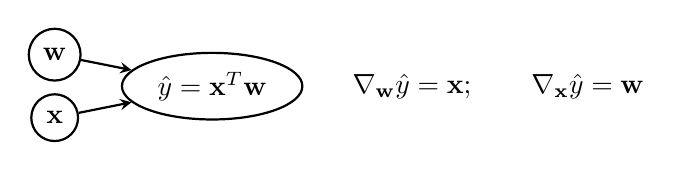
\begin{tikzpicture}
\node (x) [draw, circle, thick] at (0,0.6) {$\mathbf{x}$};
\node (w) [draw, circle, thick] at (0,1.4) {$\mathbf{w}$};
\node (dot) [draw, ellipse, thick] at (2,1) {$\hat{y} = \mathbf{x}^T \mathbf{w}$};
\node [right=5mm of dot] {$ \nabla_{\mathbf{w}} \hat{y} = \mathbf{x} ; \qquad \nabla_{\mathbf{x}} \hat{y} = \mathbf{w}$};
\draw [->, >=stealth, thick] (x) -- (dot);
\draw [->, >=stealth, thick] (w) -- (dot);
\end{tikzpicture}}
\begin{itemize}
	\item When we apply operations to tensors, pytorch implicitly builds a computation graph
	\item When backpropagation is invoked at a scalar tensor, the gradients of that tensor are computed via automatic differentiation
	\item The gradients are stored in the $\texttt{grad}$ attribute of the input tensors:
\end{itemize}
\begin{minted}[fontsize=\footnotesize,fontfamily=courier]{python}
>>> x = torch.tensor([1., 2., 3.], requires_grad=True)
>>> w = torch.tensor([0., 0., 1.], requires_grad=True)
>>> y_hat = x.dot(w)
>>> y_hat
tensor(3., grad_fn=<DotBackward>)
>>> y_hat.backward()
>>> (w.grad, x.grad)
(tensor([1., 2., 3.]), tensor([0., 0., 1.]))
\end{minted}
	
			
\vfill

\end{vbframe}

% \begin{vbframe}{Automatic differentiation}

% \center{\begin{tikzpicture}
% \node (x) [draw, circle, thick] at (0,0.6) {$\mathbf{x}$};
% \node (w) [draw, circle, thick] at (0,1.4) {$\mathbf{w}$};
% \node (dot) [draw, ellipse, thick] at (2,1) {$\hat{y} = \mathbf{x}^T \mathbf{w}$};
% \node [right=5mm of dot] {$ \nabla_{\mathbf{w}} \hat{y} = \mathbf{x} ; \qquad \nabla_{\mathbf{x}} \hat{y} = \mathbf{w}$};
% \draw [->, >=stealth, thick] (x) -- (dot);
% \draw [->, >=stealth, thick] (w) -- (dot);
% \end{tikzpicture}}
% \begin{itemize}
% 	\item When we apply operations to tensors, pytorch implicitly builds a computation graph
% 	\item When backpropagation is invoked at a scalar tensor, the gradients of that tensor are computed via automatic differentiation
% 	\item The gradients are stored in the $\texttt{grad}$ attribute of the input tensors:
% \end{itemize}
% \begin{minted}[fontsize=\footnotesize,fontfamily=courier]{python}
% >>> x = torch.tensor([1., 2., 3.], requires_grad=True)
% >>> w = torch.tensor([0., 0., 1.], requires_grad=True)
% >>> y_hat = x.dot(w)
% >>> y_hat
% tensor(3., grad_fn=<DotBackward>)
% >>> y_hat.backward()
% >>> (w.grad, x.grad)
% (tensor([1., 2., 3.]), tensor([0., 0., 1.]))
% \end{minted}
	
			
% \vfill

% \end{vbframe}
	
\begin{frame}[fragile]
\frametitle{Disabling automatic differentiation}
\begin{itemize}
	\item Automatic differentiation is expensive:
	\begin{itemize}
	\item We have to store the content of all intermediate tensors
	\item After backpropagation, we have to store the gradients
	\end{itemize}
	\item Disabling automatic differentiation:
	\begin{itemize}
	\item Use \texttt{requires\_grad=False} for tensors that do not require gradients (e.g., ``frozen'' parameters)
	\item When you don't intend to do gradient updates (e.g., during evaluation), use \texttt{torch.no\_grad()} context 
	\end{itemize}
\end{itemize}
\begin{minted}[fontsize=\scriptsize]{python}
>>> x = torch.tensor([1., 2., 3.], requires_grad=False)
>>> w = torch.tensor([0., 0., 1.], requires_grad=True)
>>> with torch.no_grad(): 
>>>   y_hat = x.dot(w)
>>>   y_hat.backward()  # no_grad context -> no backpropagation
RuntimeError
>>> y_hat = x.dot(w)
>>> y_hat.backward() 
>>> (w.grad, x.grad) # gradients only for tensors with requires_grad=True
(torch.tensor([1., 2., 3.]), None)
\end{minted}
\end{frame}
	
	

\begin{vbframe}{Automatic differentiation via chain rule: Feed-Forward Net}
\vspace{-1cm}
\center{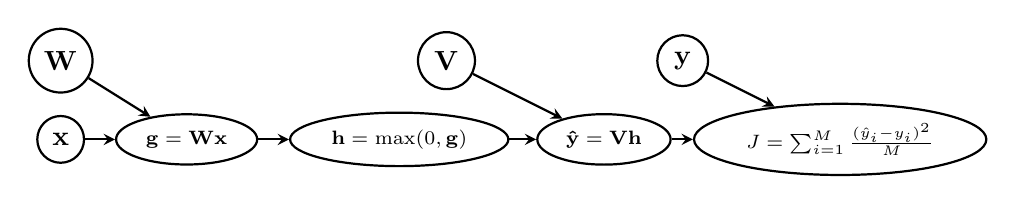
\begin{tikzpicture}
\node (x) [draw, circle, thick] at (0.1,1) {$\mathbf{x}$};
\node (w) [draw, circle, thick] at (0.1,2) {$\mathbf{W}$};
\node (g) [draw, ellipse, thick] at (1.7,1) {\scriptsize $\mathbf{g} = \mathbf{W}\mathbf{x}$};
\node (h) [draw, ellipse, thick] at (4.4,1) {\scriptsize $\mathbf{h} = \mathrm{max}(0, \mathbf{g})$};
\node (u) [draw, circle, thick] at (5,2) {$\mathbf{V}$};
\node (prob) [draw, ellipse, thick] at (7, 1) {\scriptsize $\mathbf{\hat{y}}=\mathbf{V}\mathbf{h}$};
\node (y) [draw, circle, thick] at (8, 2) {$\mathbf{y}$};
\node (nll) [draw, ellipse, thick] at (10, 1) {\scriptsize $J=\sum_{i=1}^M \frac{(\hat{y}_i - y_i)^2}{M}$};
\draw [->, >=stealth, thick] (x) -- (g);
\draw [->, >=stealth, thick] (w) -- (g);
\draw [->, >=stealth, thick] (g) -- (h);
\draw [->, >=stealth, thick] (h) -- (prob);
\draw [->, >=stealth, thick] (u) -- (prob);
\draw [->, >=stealth, thick] (y) -- (nll);
\draw [->, >=stealth, thick] (prob) -- (nll);
\end{tikzpicture}}

\begin{minted}[fontsize=\scriptsize,fontfamily=courier]{python}
>>> x = torch.tensor([1., 2., 3.], requires_grad=False) # inputs
>>> y = torch.tensor([.7, .8], requires_grad=False) # targets
>>> W = torch.rand(size=(3,2), requires_grad=True) # param 1
>>> V = torch.rand(size=(2,2), requires_grad=True) # param 2
>>> g = x.matmul(W) # hidden vector
>>> h = torch.relu(g) # hidden vector after nonlinearity
>>> y_hat = h.matmul(V) # predicted vector
>>> J = torch.mean((y_hat - y)**2) # MSE loss
>>> J.backward()
>>> W.grad
tensor([[2.1843, 1.4898],
		[4.3687, 2.9796],
		[6.5530, 4.4694]])
>>> V.grad
tensor([[3.7324, 4.8193],
		[7.0224, 9.0673]])

\end{minted}


\end{vbframe}

\begin{vbframe}{Automatic differentiation}
\vfill
\begin{itemize}
\item No matter how complicated our neural network becomes: As long as every function is a (differentiable) pytorch function, pytorch can derive the gradients via the chain rule.
\item No more manual backpropagation! 
\end{itemize}
\end{vbframe}

\begin{vbframe}{Modules}
\vfill
\begin{itemize}
\item Pytorch groups functions and their parameters into \textit{modules} (also called \textit{layers})
\item \texttt{torch.nn} contains many predefined module classes:
\end{itemize}
\begin{minted}[fontsize=\tiny,fontfamily=courier]{python}
>>> import torch.nn as nn
>>> nn.Linear(in_features, out_features) # simple linear layer
>>> nn.Conv2d(in_channels, out_channels, kernel_size) # 2D CNN
>>> nn.Embedding(num_embeddings, embedding_dim) # lookup layer
>>> # and many more
\end{minted}
\begin{itemize}
\item Here, we instantiate a linear layer with input size 3 and output size 2:
\end{itemize}
\begin{minted}[fontsize=\tiny,fontfamily=courier]{python}
>>> torch.random.manual_seed(0)
>>> linear = nn.Linear(in_features=3, out_features=2, bias=True)
\end{minted}
\end{vbframe}
	
\begin{vbframe}{Modules: parameters}
\begin{itemize}
\item Most modules have parameters
\item For example, our linear layer has a parameter matrix and a bias vector
\item The parameters are randomly initialized when the module is created
\item We can inspect the parameters:
\end{itemize}
\begin{minted}[fontsize=\tiny,fontfamily=courier]{python}
>>> list(linear.parameters())
[Parameter containing:
tensor([[-0.0043,  0.3097, -0.4752],
		[-0.4249, -0.2224,  0.1548]], requires_grad=True), 
Parameter containing:
tensor([-0.0114,  0.4578], requires_grad=True)]
\end{minted}
\begin{itemize}
\item Note that \texttt{requires\_grad} is set to \texttt{True}, because pytorch expects us to train these parameters.
\end{itemize}
\end{vbframe}
	
\begin{frame}[fragile]{Modules: \texttt{forward} function}
\begin{itemize}
\item Every module class has a \texttt{forward} function, which handles the forward-pass logic.
\item In the case of the linear layer, the forward-pass logic is simply:
$$ f(\mathbf{x}) = \mathbf{W} \mathbf{x} + \mathbf{b}$$
\end{itemize}
% # from https://pytorch.org/docs/stable/_modules/torch
\begin{minted}[fontsize=\small,fontfamily=courier,fontencoding=T1]{python}
class Linear(Module):
# (...)
def forward(self, input: Tensor) -> Tensor:
	return F.linear(input, self.weight, self.bias)
# F.linear:
def linear(input, weight, bias=None):
# (...)
output = input.matmul(weight.t())
if bias is not None:
	output += bias
ret = output
return ret
\end{minted}
\end{frame}
	
\begin{vbframe}{Modules: \texttt{forward()} function}
\begin{itemize}
\item ``Calling'' a module means calling its forward function:
\end{itemize}
\begin{minted}[fontsize=\tiny,fontfamily=courier]{python}
		>>> inputs = torch.tensor([[1., 2., 3.], [4., 5., 6.]])
		>>> predictions = linear(inputs)
		>>> predictions
		tensor([[-0.8219,  0.0526],
				[-1.3313, -1.4247]], grad_fn=<AddmmBackward>)
		>>> linear.forward(inputs) # this is equivalent
		tensor([[-0.8219,  0.0526],
				[-1.3313, -1.4247]], grad_fn=<AddmmBackward>)
\end{minted}
\vfill
\begin{itemize}
\item Typically, modules expect their inputs to have a batch axis. So in reality, the input is a tensor of shape ($N$, $\ldots$), where $N$ is the number of datapoints per batch (here: 2), and $\ldots$ stands for the remaining axes (here: one 3-dimensional feature axis).
The layer is then applied to every datapoint independently.
\end{itemize}
\end{vbframe}
	
\begin{vbframe}{Loss functions}
\begin{itemize}
\item Many popular loss functions are pre-implemented in \texttt{torch.nn}:
\end{itemize}
\begin{minted}[fontsize=\small,fontfamily=courier]{python}
>>> nn.MSELoss() # mean squared error
>>> nn.BCELoss() # Negative Log Likelihood (binary)
>>> nn.NLLLoss() # Negative Log Likelihood (multi-class)
>>> # and many more
\end{minted}
\begin{itemize}
\item A loss function behaves like a module, except that it has no parameters, and its forward function usually takes two inputs (the prediction and the target):
\end{itemize}
\begin{minted}[fontsize=\small,fontfamily=courier]{python}
>>> loss_function = nn.MSELoss()
>>> targets = torch.tensor([[.1, .2], [-.3, -.4]])
>>> predictions = linear(inputs)
>>> predictions
tensor([[-0.8219,  0.0526],
	[-1.3313, -1.4247]], grad_fn=<AddmmBackward>)
>>> loss = loss_function(predictions, targets)
>>> loss
tensor(0.7463, grad_fn=<MseLossBackward>)
\end{minted}
\end{vbframe}
	
\begin{vbframe}{Backpropagation}
\begin{itemize}
\item Now we can backpropagate the loss:
\end{itemize}
\begin{minted}[fontsize=\small,fontfamily=courier]{python}
	>>> loss.backward()
\end{minted}
\vfill
\begin{itemize}
\item Let's look at the gradients of the loss w.r.t. the parameters. There is one gradient tensor per parameter (one for the matrix and one for the bias). These gradients were calculated when we called \texttt{loss.backward()}, and they are stored in the \texttt{grad} attribute:
\end{itemize}
\begin{minted}[fontsize=\small,fontfamily=courier]{python}
>>> [param.grad for param in linear.parameters()]
[tensor([[-2.5235, -3.5000, -4.4766],
		[-2.1231, -2.7092, -3.2953]]), 
tensor([-0.9766, -0.5861])]
\end{minted}
\end{vbframe}
		
\begin{frame}[fragile]
\frametitle{Gradient update}
\vfill
\begin{itemize}
\item Now that we have the gradients, we could update the parameters manually:
\end{itemize}
\begin{minted}[fontsize=\small]{python}
>>> learning_rate = 0.01
>>> with torch.no_grad():
...   for param in linear.parameters():
...     param.sub_(learning_rate*param.grad)
\end{minted}
\begin{itemize}
\item But that's too much work.
\item Instead, we use an optimizer from the \texttt{torch.optim} package
\end{itemize}
\end{frame}

\begin{frame}[fragile]
\frametitle{Optimizers}
\vfill
\begin{itemize}
\item Optimizers are objects that take care of gradient updates.
\item When instantiating an optimizer, you pass the model parameters to it. That way, the optimizer knows what it has to update:
\end{itemize}
\begin{minted}[fontsize=\footnotesize]{python}
>>> import torch.optim as optim
>>> optimizer = optim.SGD(linear.parameters(), lr=0.01)
\end{minted}
\begin{itemize}
\item Pytorch has many complex pre-implemented optimizers
\item Complex optimizers can do things like adapt the momentum of the learning rate, use different learning rates for different parameters, etc.
\end{itemize}
\begin{minted}[fontsize=\footnotesize]{python}
>>> optim.Adam(linear.parameters(), lr=0.01)
>>> optim.RMSprop(linear.parameters(), lr=0.01)
>>> # ...and many more. Let's use SGD for now.
\end{minted}
\end{frame}
	
\begin{frame}[fragile]
\frametitle{Optimizers}
\begin{itemize}
\item With an optimizer, the gradient update step is simply:
\end{itemize}
\begin{minted}[fontsize=\footnotesize]{python}
>>> optimizer.step() # update all parameters with their gradients
>>> optimizer.zero_grad() # zero out all gradients
\end{minted}
\begin{itemize}
\item Careful: The call to \texttt{optimizer.zero\_grad()} is easy to forget. But it is important.
\begin{itemize}
\item If we don't zero out gradients, they sum up inside the \texttt{grad} tensor. As a result, the ``gradient'' at training step 1000 would be $\sum_{i=1}^{1000} \nabla_\theta J(\theta; x_i, y_i)$ instead of $\nabla_\theta J(\theta; x_{1000}, y_{1000})$ (where $x_i, y_i$ is the $i$'th training batch)
\end{itemize}
\end{itemize}
\end{frame}

\begin{frame}[fragile]
\frametitle{Using pytorch on a GPU}

\begin{itemize}
\item First, check if CUDA is available on your machine:
\end{itemize}
\begin{minted}[fontsize=\scriptsize]{python}
>>> torch.cuda.is_available()
True
\end{minted}
\begin{itemize}
\item Then, move your model (your \texttt{nn.module} object) to the GPU.
\end{itemize}
\begin{minted}[fontsize=\scriptsize]{python}
>>> model = model.to(device='cuda')
\end{minted}
\begin{itemize}
\item If you have several GPUs, you can select them by their index:
\end{itemize}
\begin{minted}[fontsize=\scriptsize]{python}
>>> model = model.to(device='cuda:2') # indices start at 0
\end{minted}
\begin{itemize}
\item Inputs have to be on the same device as the model:
\end{itemize}
\begin{minted}[fontsize=\scriptsize]{python}
>>> inputs = inputs.to(device='cuda') # or whatever device the model is on
>>> predictions = model(inputs)
\end{minted}
\begin{itemize}
\item Tensors that were computed by your model (here: \texttt{predictions}) live on the same device as the model. To move them back to the CPU:
\end{itemize}
\begin{minted}[fontsize=\scriptsize]{python}
>>> predictions.to(device='cpu')
\end{minted}
\end{frame}
	
		

\endlecture
\end{document}
